% !TEX root = ../main.tex
\section{Contextual Prototypical Memory Networks}
% !TEX root = ../main.tex
\begin{figure}[t]
\vspace{-0.7in}
\begin{minipage}[c]{0.5\linewidth}
\centering
\vspace{0.25in}
\iflatexml
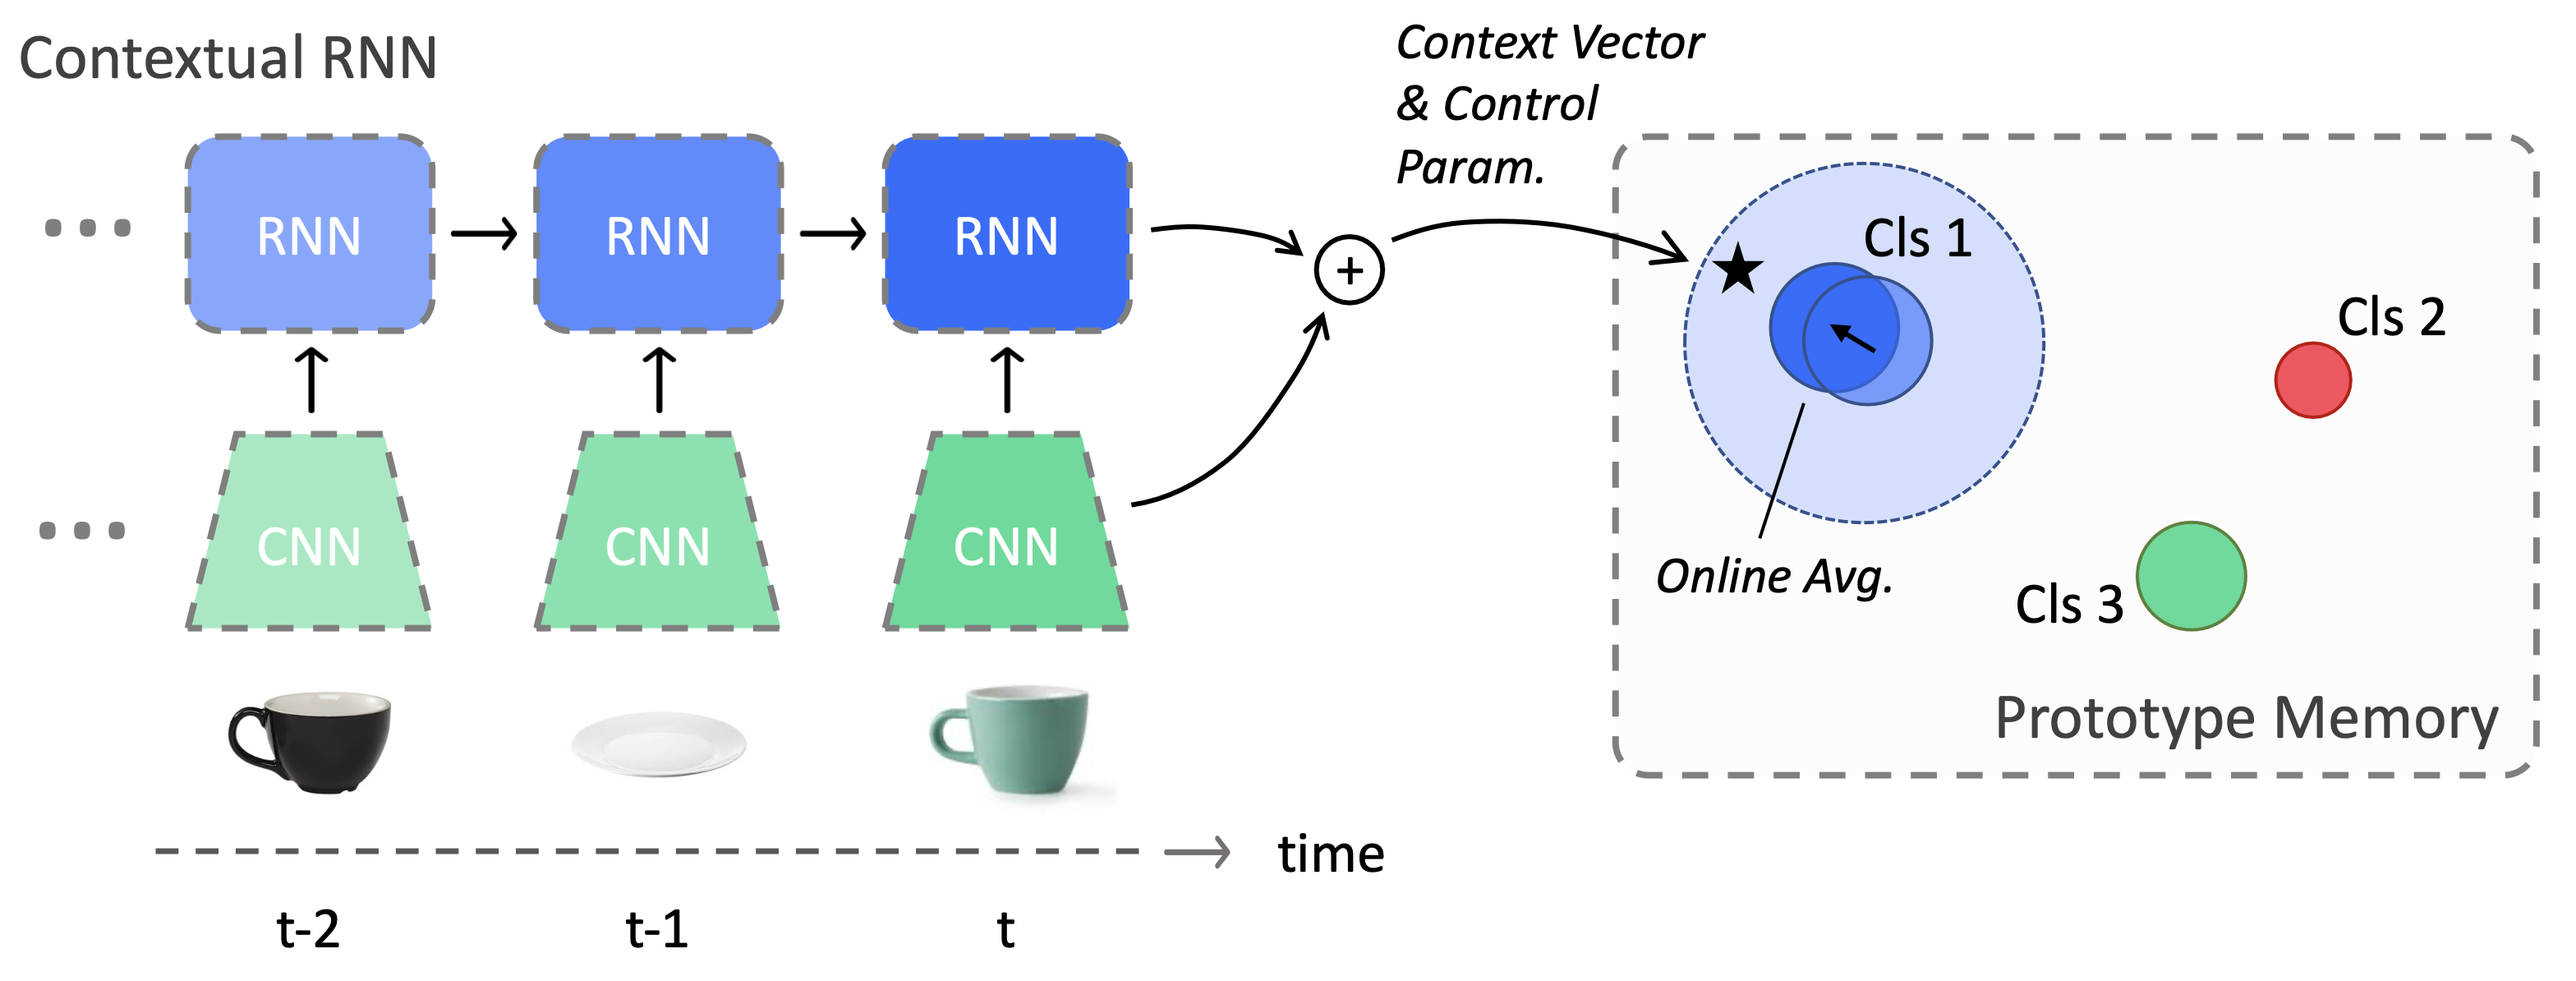
\includegraphics[width=6\linewidth]{figures/our_model.png}
\else
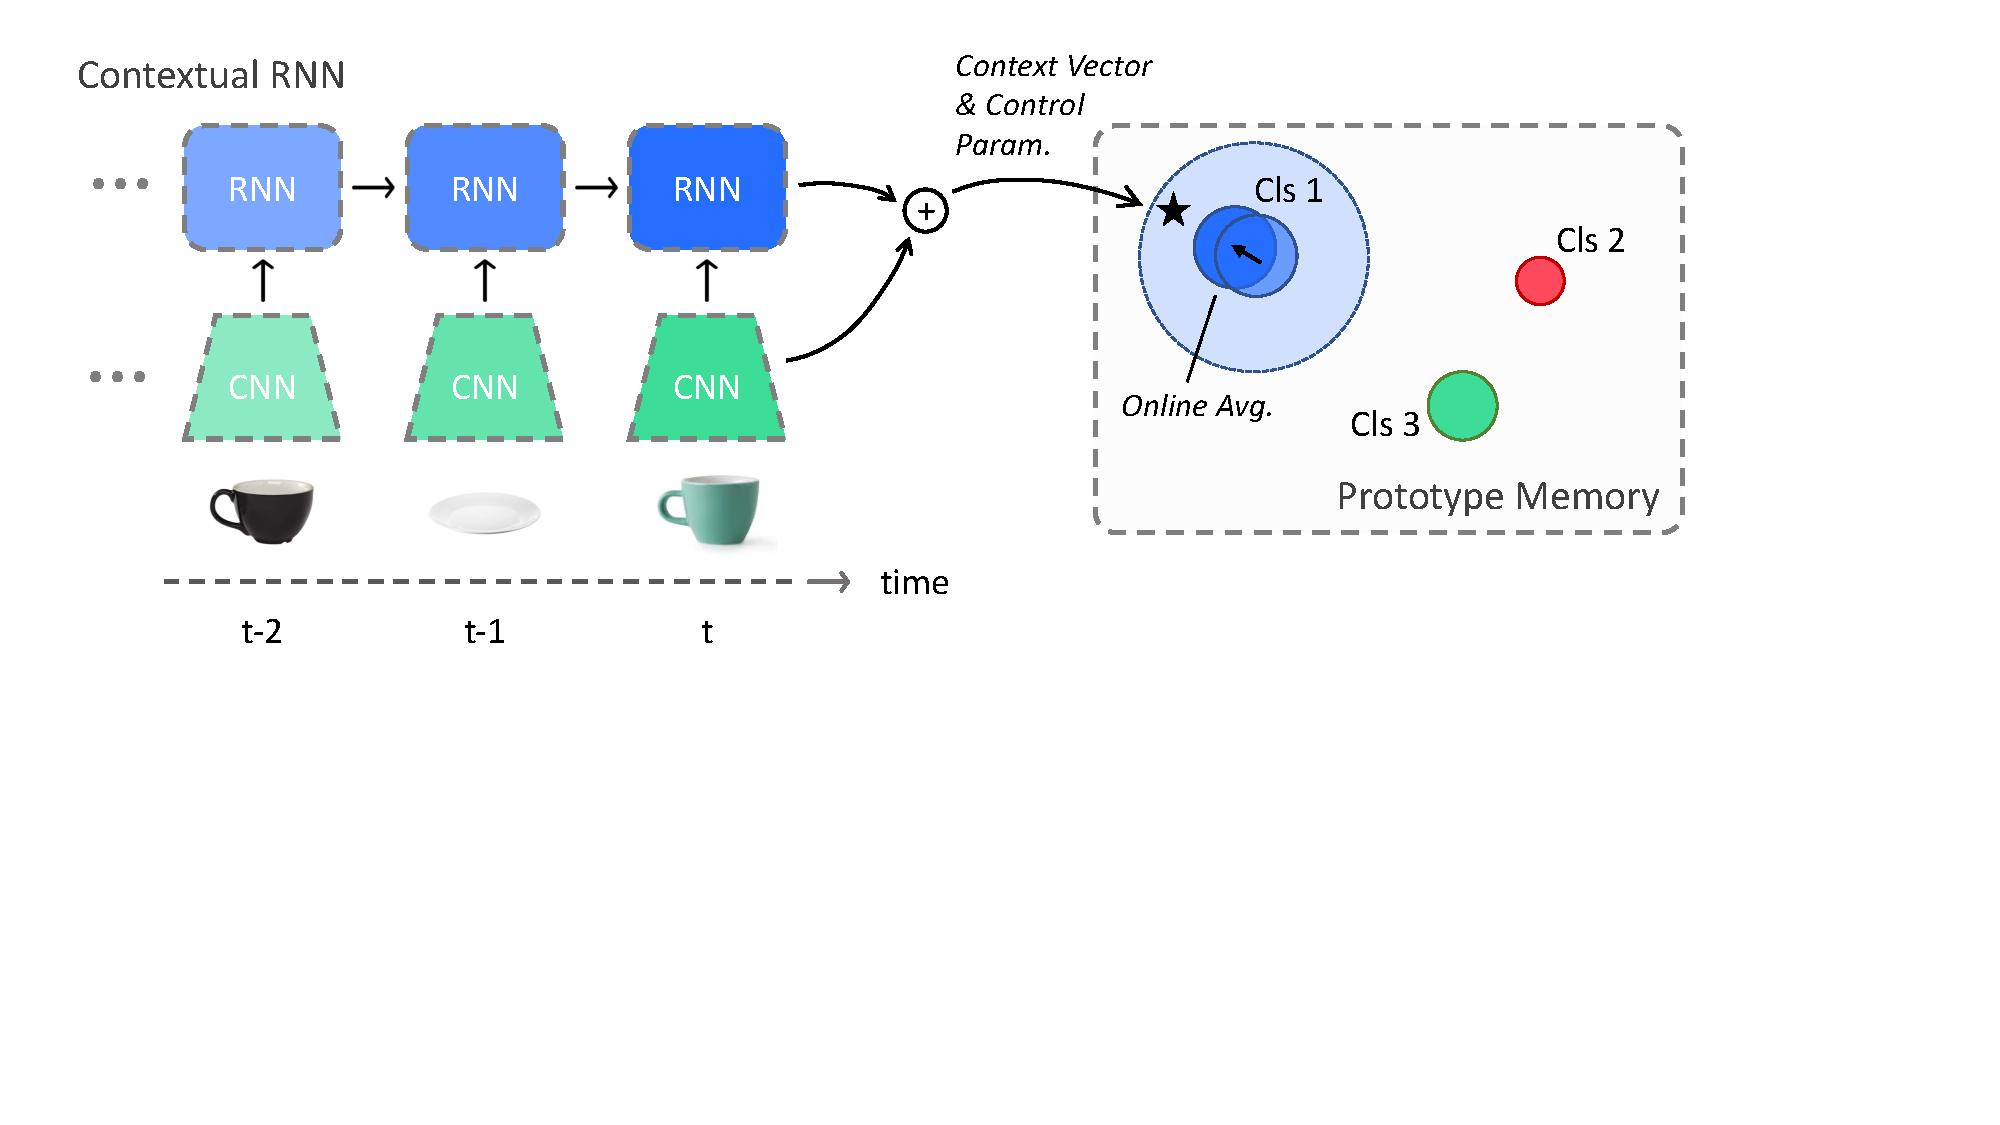
\includegraphics[width=\linewidth,trim={0 8cm 4.5cm 0.3cm},clip]{figures/our_model.pdf}
\fi
\end{minipage}
% \hfill
\begin{minipage}[c]{0.5\linewidth}
\caption{\textbf{Contextual prototypical memory.} Temporal contextual features are extracted
from an RNN. The prototype memory stores one vector per class and does online averaging.
Examples falling outside the radii of all prototypes are classified as ``new.'' }
\label{fig:mainmodel}
\end{minipage}
\vspace{-0.25in}
\end{figure}

\vspace{-0.1in}
In the online contextualized few-shot learning setup, the few-shot learner can potentially improve
by modeling the temporal context. Metric learning approaches~\citep{protonet} typically ignore
temporal contextual relations and directly compare the similarity between training and test samples.
Gradient-based approaches~\citep{oml}, on the other hand, have the ability to adapt to new contexts,
but they do not naturally handle new and unlabeled examples. Inspired by the
contextual binding theory of human memory ~\citep{ctxbinding}, we propose a simple yet effective
approach that uses an RNN to transmit spatiotemporal context and control signals to a prototype memory
(Figure~\ref{fig:mainmodel}).

% Next, we describe our approach in detail.
% augments the classic Prototypical Network with a temporal
% contextual encoder using an RNN, shown in Figure~\ref{fig:mainmodel}. Next, we describe our approach
% in detail. \MR{Edit augment, emphasize interaction, add neuroscience paper}

\vspace{-0.1in} \paragraph{Prototype memory:} We start describing our model with the prototype
memory, which is an online version of the Prototypical Network (or
\emph{ProtoNet})~\citep{protonet}. ProtoNet can be viewed as a knowledge base memory, where each
object class $k$ is represented by a prototype vector $\bp[k]$, computed as the mean vector of all
the support instances of the class in a sequence. It can also be applied to our task of online
few-shot learning naturally, with some modifications. Suppose that at time-step $t$ we have already
stored a few classes in the memory, each represented by their current prototype $\bp_t[k]$, and we
would like to query the memory using the input feature $\bh_t$. We model our prototype memory as %
% \vskip -0.60cm % \begin{align} % 
% $\hat{y}_{t,k}   &= \softmax( -\lVert \bh_t- \bp_t[k]
% \rVert^2_{\bM_t})$, 
$\hat{y}_{t,k} = \softmax( -d_{\bmm_t}(\bh_t, \bp_t[k]))$, % \end{align} %
% \vskip -0.30cm % the squared Mahalanobis distance for  where $d_{\bmm_t}$ is a dissimilarity score
(e.g. squared Euclidean distance or cosine dissimilarity) parameterized by a vector $\bmm_t$ that
scales each dimension with a Hadamard product. To predict whether an example is of a new class, we
can use a separate \emph{novelty} output $\hat{u}_t^{r}$ with sigmoid activation, similar to the
approach introduced in~\citet{fewshotssl}, where $\beta_t^r$ and $\gamma_t^r$ are
yet-to-be-specified thresholding hyperparameters (the superscript $r$ stands for read): 
\vskip -0.5cm 
\begin{align}
\hat{u}_t^{r} &= \sigmoid( (\min_k d_{\bmm_t}(\bh_t, \bp_t[k]) - \beta_t^r) /
\gamma_t^r).
\label{eq:ur}
\end{align}
\vskip -0.25cm

% \renewcommand{\sidecaptionsep}{2mm}

\vspace{-0.1in}
\paragraph{Memory consolidation with online prototype averaging:}
Traditionally, ProtoNet uses the average representation of a class across all support examples.
Here, we must be able to adapt the prototype memory incrementally at each step. 
% Fortunately, we are
% able to recover the same prototypes as a regular ProtoNet computes offline by using online
% averaging. For each prototype $k$, we store a count scalar $c[k]_t$ to 
Fortunately, we can recover the computation of a ProtoNet by performing a simple online averaging:
\vskip -0.8cm
\begin{align}
c_t &= c_{t-1} + 1; \ \ A(\bh_t; \bp_{t-1}, c_t) = \frac{1}{c_t} \left( \bp_{t-1} c_{t-1} +\bh_t \right),
\end{align}
\vskip -0.3cm
where $\bh$ is the input feature, and $\bp$ is the prototype, and $c$ is a scalar indicating the
number of examples that have been added to this prototype up to time $t$. The online averaging function
$A$ can also be made more flexible to allow more plasiticity, modeled by a
\textit{gated averaging unit} (GAU):
\vskip -0.5cm
\begin{align}
A_{\text{GAU}}(\bh_t; \bp_{t-1}) &= (1-f_t) \cdot \bp_{t-1} + f_t \cdot \bh_t, \ \ \ \text{where} \
\ f_t = \sigmoid(W_f [\bh_t, \bp_{t-1}] + b_f) \in \mathbb{R}.
\end{align}
\vskip -0.25cm
When the current example is
unlabeled, $\tilde{y}_t$ is encoded as $-1$, and the model's own prediction $\hat{y}_t$ will determine
which prototype to update; in this case, the model must also determine a strength of belief,
$\hat{u}_t^w$, that the current unlabeled example should be treated as a new class.  Given
$\hat{u}_t^w$ and $\hat{y}_t$, the model can then update a prototype:
\vskip -0.5cm
\begin{align}
% \hat{u}_t^{w} &= \sigmoid((\min_k \lVert \bh_t - \bp_t[k] \rVert^2_{\bM_t} - \beta_t^w) /
\hat{u}_t^{w} &= \sigmoid((\min_k d_{\bmm_t}(\bh_t, \bp_t[k]) - \beta_t^w) / \gamma_t^w),\\
\Delta[k]_t   &= \underbrace{\mathbbm{1}[\tilde{y}_t = k]}_{\text{Supervised}} +
             \underbrace{\hat{y}_{t,k} (1 - \hat{u}_t^{w}) \mathbbm{1}[\tilde{y}_t =
-1]}_{\text{Unsupervised}}, \\ c[k]_t        &= c[k]_{t-1} + \Delta[k]_t,\\
\bp[k]_t      &= A(\bh_{t} \Delta[k]_t; \bp[k]_{t-1}, c[k]_t), \ \ \text{or} \ \ \bp[k]_t = A_{\text{GAU}}(\bh_{t} \Delta[k]_t; \bp[k]_{t-1}).
% \bp[k]_t      &= \frac{1}{c[k]_t} \left( \bp[k]_{t-1} c[k]_{t-1} +\bh_{t} \Delta[k]_t \right) \ \
% \text{if} \ \ \Delta[k]_t > 0.
\end{align}
% where $A$ is an online mean that computes prototypes.
\looseness=-1
As-yet-unspecified hyperparameters $\beta_t^w$ and $\gamma_t^w$ are required (the superscript $w$
%in $\beta_t^w$ and $\gamma_t^w$ 
is for write). These parameters for the online-updating novelty
output $\hat{u}_t^{w}$ are  distinct from $\beta_t^r$ and $\gamma_t^r$ in Equation~\ref{eq:ur}. The
intuition is that for ``self-teaching'' to work, the model potentially needs to be more conservative
in creating new classes (avoiding corruption of prototypes) than in predicting an input as being a
new class.

% !TEX root = ../main.tex
\begin{table}[t]
\begin{center}
\vspace{-0.5in}
\caption{\textbf{\ourchar{} OC-FSL results.} Max 5 env, 150 images, 50 cls, with 8$\times$8 occlusion.}
\label{tab:omniglot}
\iflatexml
\begin{tabular}{cccc|ccc}
\toprule
\mr{2}{\tb{Method}} & \mc{3}{c|}{\tb{Supervised}}                         &  \mc{3}{c}{\tb{Semi-supervised}}            \\
                     & AP         & 1-shot Acc.           & 3-shot Acc.           & AP         & 1-shot Acc.           & 3-shot Acc.           \\
\midrule         
LSTM                 & 64.34      & 61.00 $\pm$ 0.22      & 81.85 $\pm$ 0.21      & 54.34      & 68.30 $\pm$ 0.20      & 76.38 $\pm$ 0.49      \\
DNC                  & 81.30      & 78.87 $\pm$ 0.19      & 91.01 $\pm$ 0.15      & 81.37      & 88.56 $\pm$ 0.12      & 93.81 $\pm$ 0.26      \\
OML-U                & 77.38      & 70.98 $\pm$ 0.21      & 89.13 $\pm$ 0.16      & 66.70      & 74.65 $\pm$ 0.19      & 90.81 $\pm$ 0.34      \\
OML-U++              & 86.85      & 88.43 $\pm$ 0.14      & 92.01 $\pm$ 0.14      & 81.39      & 71.64 $\pm$ 0.19      & 93.72 $\pm$ 0.27      \\
\OnlineMatchingNet{} & 88.69      & 84.82 $\pm$ 0.15      & 95.55 $\pm$ 0.11      & 84.39      & 88.77 $\pm$ 0.13      & 97.28 $\pm$ 0.17      \\
\OnlineIMP{}         & 90.15      & 85.74 $\pm$ 0.15      & 96.66 $\pm$ 0.09      & 81.62      & 88.68 $\pm$ 0.13      & 97.09 $\pm$ 0.19      \\
\OnlineProtoNet{}    & 90.49      & 85.68 $\pm$ 0.15      & 96.95 $\pm$ 0.09      & 84.61      & 88.71 $\pm$ 0.13      & 97.61 $\pm$ 0.17      \\
CPM (Ours)           & \tb{94.17} & \tb{91.99} $\pm$ 0.11 & \tb{97.74} $\pm$ 0.08 & \tb{90.42}      & \tb{93.18} $\pm$ 0.16      & \tb{97.89} $\pm$ 0.15      \\
\bottomrule
\end{tabular}
\else
\begin{small}
\resizebox{.75\textwidth}{!}{
\begin{tabular}{cccc|ccc}
\toprule
\mr{2}{\tb{Method}} & \mc{3}{c|}{\tb{Supervised}}                         &  \mc{3}{c}{\tb{Semi-supervised}}            \\
                     & AP         & 1-shot Acc.           & 3-shot Acc.           & AP         & 1-shot Acc.           & 3-shot Acc.           \\
\midrule         
LSTM                 & 64.34      & 61.00 $\pm$ 0.22      & 81.85 $\pm$ 0.21      & 54.34      & 68.30 $\pm$ 0.20      & 76.38 $\pm$ 0.49      \\
DNC                  & 81.30      & 78.87 $\pm$ 0.19      & 91.01 $\pm$ 0.15      & 81.37      & 88.56 $\pm$ 0.12      & 93.81 $\pm$ 0.26      \\
OML-U                & 77.38      & 70.98 $\pm$ 0.21      & 89.13 $\pm$ 0.16      & 66.70      & 74.65 $\pm$ 0.19      & 90.81 $\pm$ 0.34      \\
OML-U++              & 86.85      & 88.43 $\pm$ 0.14      & 92.01 $\pm$ 0.14      & 81.39      & 71.64 $\pm$ 0.19      & 93.72 $\pm$ 0.27      \\
\OnlineMatchingNet{} & 88.69      & 84.82 $\pm$ 0.15      & 95.55 $\pm$ 0.11      & 84.39      & 88.77 $\pm$ 0.13      & 97.28 $\pm$ 0.17      \\
\OnlineIMP{}         & 90.15      & 85.74 $\pm$ 0.15      & 96.66 $\pm$ 0.09      & 81.62      & 88.68 $\pm$ 0.13      & 97.09 $\pm$ 0.19      \\
\OnlineProtoNet{}    & 90.49      & 85.68 $\pm$ 0.15      & 96.95 $\pm$ 0.09      & 84.61      & 88.71 $\pm$ 0.13      & 97.61 $\pm$ 0.17      \\
CPM (Ours)           & \tb{94.17} & \tb{91.99} $\pm$ 0.11 & \tb{97.74} $\pm$ 0.08 & \tb{90.42}      & \tb{93.18} $\pm$ 0.16      & \tb{97.89} $\pm$ 0.15      \\
\bottomrule
\end{tabular}
}
% \vspace{-0.1in}
\end{small}
\fi
\end{center}
\end{table}

% !TEX root = ../main.tex
\begin{table}[t]
\vspace{-0.15in}
\caption{\textbf{\ourroom{} OC-FSL results.} Max 100 images and 40 classes.}
\begin{center}
\iflatexml
    \begin{tabular}{cccc|ccc}
    \toprule
    \mr{2}{\tb{Method}}  & \mc{3}{c|}{\tb{Supervised}}                                &  \mc{3}{c}{\tb{Semi-supervised}}                          \\
                         & AP         & 1-shot Acc.           & 3-shot Acc.           & AP         & 1-shot Acc.           & 3-shot Acc.          \\
    \midrule
    LSTM                 & 45.67      & 59.90 $\pm$ 0.40      & 61.85 $\pm$ 0.45      & 33.32      & 52.71 $\pm$ 0.38      & 55.83 $\pm$ 0.76     \\
    DNC                  & 80.86      & 82.15 $\pm$ 0.32      & 87.30 $\pm$ 0.30      & 73.49      & 80.27 $\pm$ 0.33      & 87.87 $\pm$ 0.49     \\
    % OML                  & 74.34      & 72.63 $\pm$ 0.37      & 84.97 $\pm$ 0.32      & 58.71      & 68.87 $\pm$ 0.38      & 87.62 $\pm$ 0.51     \\
    OML-U                & 76.27      & 73.91 $\pm$ 0.37      & 83.99 $\pm$ 0.33      & 63.40      & 70.67 $\pm$ 0.38      & 85.25 $\pm$ 0.56      \\
    OML-U++              & 88.03      & 88.32 $\pm$ 0.27      & 89.61 $\pm$ 0.29      & 81.90      & 84.79 $\pm$ 0.31      & 89.80 $\pm$ 0.47      \\
    \OnlineMatchingNet{} & 85.91      & 82.82 $\pm$ 0.32      & 89.99 $\pm$ 0.26      & 78.99      & 80.08 $\pm$ 0.34      & \tb{92.43} $\pm$ 0.41 \\
    \OnlineIMP{}         & 87.33      & 85.28 $\pm$ 0.31      & 90.83 $\pm$ 0.25      & 75.36      & 84.57 $\pm$ 0.31      & 91.17 $\pm$ 0.43     \\
    \OnlineProtoNet{}    & 86.01      & 84.89 $\pm$ 0.31      & 89.58 $\pm$ 0.28      & 76.36      & 80.67 $\pm$ 0.34      & 88.83 $\pm$ 0.49     \\
    CPM (Ours)           & \tb{89.14} & \tb{88.39} $\pm$ 0.27 & \tb{91.31} $\pm$ 0.26 & \tb{84.12} & \tb{86.17} $\pm$ 0.30 & 91.16 $\pm$ 0.44     \\
    \bottomrule
    \end{tabular}
    \label{tab:matterport}
\else
    \begin{small}
    \resizebox{.75\textwidth}{!}{
    \begin{tabular}{cccc|ccc}
    \toprule
    \mr{2}{\tb{Method}}  & \mc{3}{c|}{\tb{Supervised}}                                &  \mc{3}{c}{\tb{Semi-supervised}}                          \\
                         & AP         & 1-shot Acc.           & 3-shot Acc.           & AP         & 1-shot Acc.           & 3-shot Acc.          \\
    \midrule
    LSTM                 & 45.67      & 59.90 $\pm$ 0.40      & 61.85 $\pm$ 0.45      & 33.32      & 52.71 $\pm$ 0.38      & 55.83 $\pm$ 0.76     \\
    DNC                  & 80.86      & 82.15 $\pm$ 0.32      & 87.30 $\pm$ 0.30      & 73.49      & 80.27 $\pm$ 0.33      & 87.87 $\pm$ 0.49     \\
    % OML                  & 74.34      & 72.63 $\pm$ 0.37      & 84.97 $\pm$ 0.32      & 58.71      & 68.87 $\pm$ 0.38      & 87.62 $\pm$ 0.51     \\
    OML-U                & 76.27      & 73.91 $\pm$ 0.37      & 83.99 $\pm$ 0.33      & 63.40      & 70.67 $\pm$ 0.38      & 85.25 $\pm$ 0.56      \\
    OML-U++              & 88.03      & 88.32 $\pm$ 0.27      & 89.61 $\pm$ 0.29      & 81.90      & 84.79 $\pm$ 0.31      & 89.80 $\pm$ 0.47      \\
    \OnlineMatchingNet{} & 85.91      & 82.82 $\pm$ 0.32      & 89.99 $\pm$ 0.26      & 78.99      & 80.08 $\pm$ 0.34      & \tb{92.43} $\pm$ 0.41 \\
    \OnlineIMP{}         & 87.33      & 85.28 $\pm$ 0.31      & 90.83 $\pm$ 0.25      & 75.36      & 84.57 $\pm$ 0.31      & 91.17 $\pm$ 0.43     \\
    \OnlineProtoNet{}    & 86.01      & 84.89 $\pm$ 0.31      & 89.58 $\pm$ 0.28      & 76.36      & 80.67 $\pm$ 0.34      & 88.83 $\pm$ 0.49     \\
    CPM (Ours)           & \tb{89.14} & \tb{88.39} $\pm$ 0.27 & \tb{91.31} $\pm$ 0.26 & \tb{84.12} & \tb{86.17} $\pm$ 0.30 & 91.16 $\pm$ 0.44     \\
    \bottomrule
    \end{tabular}
    }
    \label{tab:matterport}
    \vspace{-0.25in}
    \end{small}
\fi
\end{center}
\end{table}

\begin{table}[t]
\vspace{-0.5in}
\caption{\textbf{\ourimg{} OC-FSL results.} Max 150 images and 50 classes. * denotes CNN pretrained using regular classification.}
\begin{center}
\iflatexml
    \begin{tabular}{cccc|ccc}
    \toprule
    \mr{2}{\tb{Method}}  & \mc{3}{c|}{\tb{Supervised}}                                &  \mc{3}{c}{\tb{Semi-supervised}}                          \\
                         & AP         & 1-shot Acc.           & 3-shot Acc.           & AP         & 1-shot Acc.           & 3-shot Acc.          \\
    \midrule
    % LSTM                 & 7.73       & 11.60 $\pm$ 0.12      & 43.93 $\pm$ 0.27      & 4.03       & 22.53 $\pm$ 0.18      & 41.34 $\pm$ 0.55     \\
    LSTM*                & 22.54      & 28.14 $\pm$ 0.20      & 52.07 $\pm$ 0.27      & 13.50      & 30.02 $\pm$ 0.20      & 46.95 $\pm$ 0.56     \\
    % DNC                  & 7.20       & 10.55 $\pm$ 0.11      & 42.22 $\pm$ 0.27      & 3.66       & 22.37 $\pm$ 0.18      & 37.83 $\pm$ 0.54     \\
    DNC*                 & 26.80      & 33.45 $\pm$ 0.19      & 55.78 $\pm$ 0.27      & 16.50      & 39.53 $\pm$ 0.19      & 54.10 $\pm$ 0.54     \\
    OML-U                & 21.89      & 15.06 $\pm$ 0.14      & 52.52 $\pm$ 0.27      & 10.16      & 22.74 $\pm$ 0.17      & 55.81 $\pm$ 0.55     \\
    % OML-U Cos            & 10.87      & 24.45 $\pm$ 0.18      & 30.89 $\pm$ 0.24      & 5.65       & 23.37 $\pm$ 0.16      & 32.79 $\pm$ 0.50     \\
    \OnlineMatchingNet{} & 13.05      & 20.61 $\pm$ 0.15      & 38.73 $\pm$ 0.24      & 9.32       & 25.96 $\pm$ 0.16      & 55.32 $\pm$ 0.51     \\
    \OnlineIMP{}         & 14.25      & 22.92 $\pm$ 0.16      & 41.01 $\pm$ 0.25      & 4.55       & 20.70 $\pm$ 0.15      & 51.23 $\pm$ 0.53     \\
    % \OnlineProtoNet{}    & 15.51      & 22.95 $\pm$ 0.17      & 44.98 $\pm$ 0.25      & 7.10       & 26.87 $\pm$ 0.16      & 42.40 $\pm$ 0.52     \\
    \OnlineProtoNet{}*   & 23.10      & 32.82 $\pm$ 0.19      & 49.98 $\pm$ 0.25      & 15.76      & 36.69 $\pm$ 0.18      & 55.47 $\pm$ 0.53     \\
    CPM (Ours)           & \tb{34.43} & \tb{40.40} $\pm$ 0.21 & \tb{60.29} $\pm$ 0.26 & \tb{24.75} & \tb{44.58} $\pm$ 0.21 & \tb{58.72} $\pm$ 0.53\\
    \bottomrule
    \end{tabular}
    \label{tab:imagenet}
\else
    \begin{small}
    \resizebox{.75\textwidth}{!}{
    \begin{tabular}{cccc|ccc}
    \toprule
    \mr{2}{\tb{Method}}  & \mc{3}{c|}{\tb{Supervised}}                                &  \mc{3}{c}{\tb{Semi-supervised}}                          \\
                         & AP         & 1-shot Acc.           & 3-shot Acc.           & AP         & 1-shot Acc.           & 3-shot Acc.          \\
    \midrule
    % LSTM                 & 7.73       & 11.60 $\pm$ 0.12      & 43.93 $\pm$ 0.27      & 4.03       & 22.53 $\pm$ 0.18      & 41.34 $\pm$ 0.55     \\
    LSTM*                & 22.54      & 28.14 $\pm$ 0.20      & 52.07 $\pm$ 0.27      & 13.50      & 30.02 $\pm$ 0.20      & 46.95 $\pm$ 0.56     \\
    % DNC                  & 7.20       & 10.55 $\pm$ 0.11      & 42.22 $\pm$ 0.27      & 3.66       & 22.37 $\pm$ 0.18      & 37.83 $\pm$ 0.54     \\
    DNC*                 & 26.80      & 33.45 $\pm$ 0.19      & 55.78 $\pm$ 0.27      & 16.50      & 39.53 $\pm$ 0.19      & 54.10 $\pm$ 0.54     \\
    OML-U                & 21.89      & 15.06 $\pm$ 0.14      & 52.52 $\pm$ 0.27      & 10.16      & 22.74 $\pm$ 0.17      & 55.81 $\pm$ 0.55     \\
    % OML-U Cos            & 10.87      & 24.45 $\pm$ 0.18      & 30.89 $\pm$ 0.24      & 5.65       & 23.37 $\pm$ 0.16      & 32.79 $\pm$ 0.50     \\
    \OnlineMatchingNet{} & 13.05      & 20.61 $\pm$ 0.15      & 38.73 $\pm$ 0.24      & 9.32       & 25.96 $\pm$ 0.16      & 55.32 $\pm$ 0.51     \\
    \OnlineIMP{}         & 14.25      & 22.92 $\pm$ 0.16      & 41.01 $\pm$ 0.25      & 4.55       & 20.70 $\pm$ 0.15      & 51.23 $\pm$ 0.53     \\
    % \OnlineProtoNet{}    & 15.51      & 22.95 $\pm$ 0.17      & 44.98 $\pm$ 0.25      & 7.10       & 26.87 $\pm$ 0.16      & 42.40 $\pm$ 0.52     \\
    \OnlineProtoNet{}*   & 23.10      & 32.82 $\pm$ 0.19      & 49.98 $\pm$ 0.25      & 15.76      & 36.69 $\pm$ 0.18      & 55.47 $\pm$ 0.53     \\
    CPM (Ours)           & \tb{34.43} & \tb{40.40} $\pm$ 0.21 & \tb{60.29} $\pm$ 0.26 & \tb{24.75} & \tb{44.58} $\pm$ 0.21 & \tb{58.72} $\pm$ 0.53\\
    \bottomrule
    \end{tabular}
    }
    \vspace{-0.2in}
    \label{tab:imagenet}
    \end{small}
\fi
\end{center}
\end{table}


\vspace{-0.1in}
\paragraph{Contextual RNN:}
Instead of directly using the features from the CNN $\bh_t^{\text{CNN}}$ as input features to the
prototype memory, we would also like to use contextual information from the recent past. Above we
introduced threshold hyperparameters $\beta_t^r$, $\gamma_t^r$, $\beta_t^w$, $\gamma_t^w$ as well as
the metric parameter $\bM_t$. We let the contextual RNN output these additional control parameters,
so that the unknown thresholds and metric function can adapt based on the information in the
context. The RNN produces the context vector $\bh_t^{\text{RNN}}$ and other control parameters
conditioned on  $\bh_t^{\text{CNN}}$:
\begin{align}
\left[ \bz_t, \bh_t^{\text{RNN}}, \bmm_t, \ \beta^r_t, \ \gamma^r_t, \ \beta^w_t, \ \gamma^w_t
\right] =
\RNN(\bh_t^{\text{CNN}}; \bz_{t-1}),
\end{align}
where $\bz_t$ is the recurrent state of the RNN, and $\bmm_t$ is the scaling factor in the
dissimilarity score. The context, $\bh_t^{\text{RNN}}$, serves as an additive bias on the state
vector used for FSL: $\bh_t  = \bh_t^{\text{CNN}} + \bh_t^{\text{RNN}}$. This addition operation in
the feature space can help contextualize prototypes based on temporal proximity, and is also similar
to how the human brain leverages spatiotemporal context for memory storage~\citep{ctxbinding}.


\vspace{-0.1in}
\paragraph{Loss function:}
The loss function is computed after an entire sequence ends and all network parameters are learned
end-to-end. The loss is composed of two parts. The first is binary cross-entropy (BCE), for telling
whether each example has been assigned a label or not, i.e., prediction of new classes, and $u_t$ is the ground-truth binary label. Second we
use a multi-class cross-entropy for classifying among the known ones. We can write down the overall
loss function as follows:
\vskip -0.5cm
\begin{align}
\cL = \frac{1}{T} \sum_{t=1}^{T}
  \lambda \underbrace{ \left[ 
- u_t \log(\hat{u}_t^r) 
- (1-u_t) \log(1 - \hat{u}_t^r)  
\right]}_{\text{Binary cross entropy on old vs. new}}
+ \sum_{k=1}^{K} \underbrace{-\mathbbm{1}[y_t = k] (1-u_t) \log(\hat{y}_{t,k})}_{\text{Cross entropy on old classes}}
.
\label{eq:loss}
\end{align}

\vspace{-0.1in}
\paragraph{Training and evaluation:} During training, we sample learning sequences and for each sequence, we perform one iterative update to minimize the loss function (Eq.~\ref{eq:loss}). At the beginning of each sequence, the memory is reset. During training, the model learns from a set of training classes. During test time, the model recognizes new classes that have never been seen during training.